\section{Introduction}

\begin{figure}
    \centering
    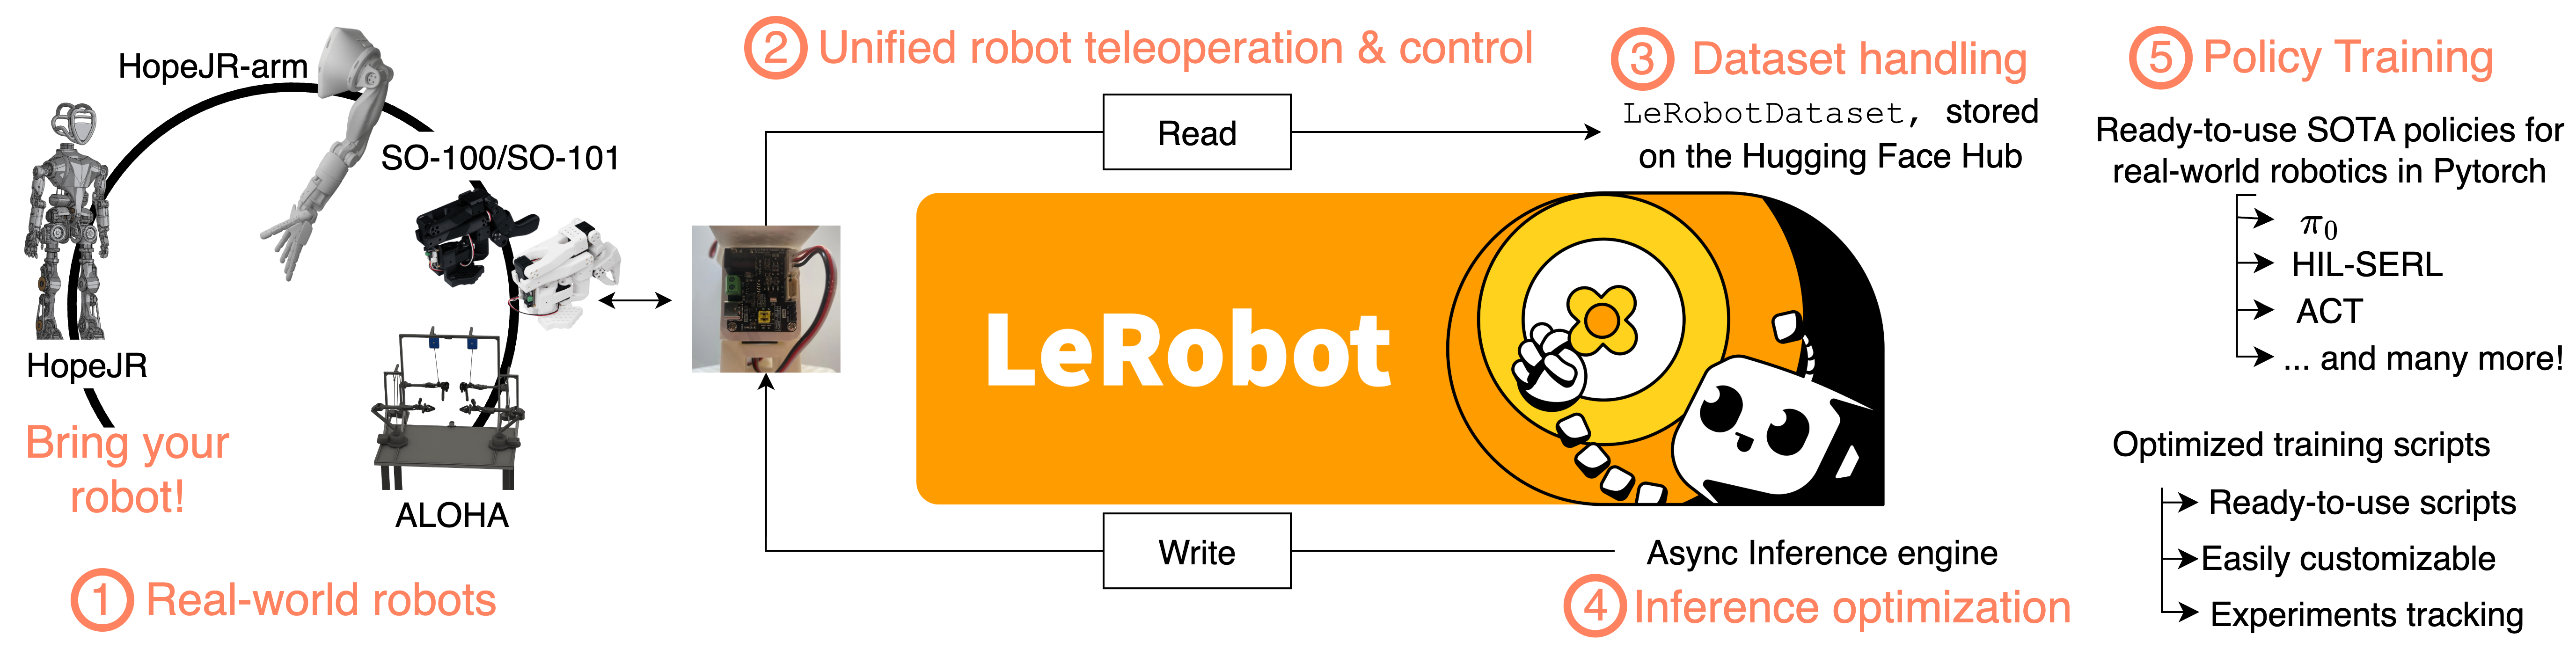
\includegraphics[width=\linewidth]{figures/ch1/ch1-lerobot-figure1.png}
    \caption{\lerobot~is the open-source library for end-to-end robotics developed by Hugging Face. The library is vertically integrated on the entire robotics stack, supporting low-level control of real-world robot devices, advanced data and inference optimizations, as well as  SOTA robot learning methods with simple implementations in pure Pytorch.}
    \label{fig:figure1}
\end{figure}

Autonomous robotics holds the premise of relieving humans from repetitive, tiring or dangerous manual tasks.
Consequently, the field of robotics has been widely studied since its first inception in the 1950s.
Lately, advancements in Machine Learning (ML) have sparked the development of a relatively new class of methods used to tackle robotics problems, leveraging large amounts of data and computation rather than human expertise and modeling skills to develop autonomous systems.

The frontier of robotics research is indeed increasingly moving away from classical model-based control paradigm, embracing the advancements made in ML, aiming to unlock (1) monolithic perception-to-action control pipelines and (2) multi-modal data-driven feature extraction strategies, together with (3) reduced reliance on precise models of the world and (4) a better positioning to benefit from the growing availability of open robotics data.
While central problems in manipulation, locomotion and whole-body control demand knowledge of rigid-body dynamics, contact modeling, planning under uncertainty, recent results seem to indicate learning can prove just as effective as explicit modeling, sparking interest in the field of \emph{robot learning}.
This interest can be largely justified considering the significant challenges related to deriving accurate models of robot-environment interactions.

Moreover, since end-to-end learning on ever-growing collections of text and image data has historically been at the core of the development of \emph{foundation models} capable of semantic reasoning across multiple modalities (images, text, audio, etc.), deriving robotics methods grounded in learning appears particularly consequential, especially as the number of openly available datasets continues to grow.

Robotics is, at its core, an inherently multidisciplinary field, requiring a wide range of expertise in both \emph{software} and \emph{hardware}.
The integration of learning-based techniques further broadens this spectrum of skills, raising the bar for both research and practical applications.
\lerobot~is an open-source library designed to integrate end-to-end with the entire robotics stack.
With a strong focus on accessible, real-world robots \highlight{(1) \lerobot~supports many, openly available, robotic platforms} for manipulation, locomotion and even whole-body control.
\lerobot also implements a \highlight{(2) unified, low-level approach to reading/writing robot configurations} to extend support for other robot platforms with relatively low effort. 
The library introduces \lerobotdataset, \highlight{(3) a native robotics dataset's format} currently being used by the community to efficiently record and share datasets.
\lerobot~also supports many state-of-the-art (SOTA) algorithms in robot learning---mainly based on Reinforcement Learning (RL) and Behavioral Cloning (BC) techniques---with efficient implementations in Pytorch, and extended support to experimentation and experiments tracking.
Lastly, \lerobot~defines a custom, optimized inference stack for robotic policies decoupling action planning from action execution, proving effective in guaranteeing more adaptability at runtime.

This tutorial serves the double purpose of providing useful references for the Science behind---and practical use of---common robot learning techniques.
To this aim, we strike to provide a rigorous yet concise overview of the core concepts behind the techniques presented, paired with practical examples of how to use such techniques concretely, with code examples in \lerobot, for researchers and practitioners interested in the field of robot learning.
This tutorial is structured as follows:
\begin{itemize}
\item Section~\ref{sec:classical} reviews classical robotics foundations, introducing the limitations of dynamics-based approaches to robotics.
\item Section~\ref{sec:learning-rl} elaborates on the limitations of dynamics-based methods, and introduce RL as a practical approach to solve robotics problems, considering its upsides and potential limitations.
\item Section~\ref{sec:learning-imitation} further describes robot learning techniques that aim at solving single-tasks learning, leveraging BC techniques to autonomously reproduce specific expert demonstrations.
\item Section~\ref{sec:learning-foundation} presents recent contributions on developing generalist models for robotics applications, by learning from large corpora of multi-task \& multi-robot data (\emph{robotics foundation models}).
% \item Lastly, Section~\ref{sec:extensions} covers emerging directions in robot learning research, introducing recent works in post-training techniques for robotics foundation models, as well as recent works in world models for robotics.
\end{itemize}

Our goal with this tutorial is to provide an intuitive explanation of the reasons various disparate ideas from Machine Learning (ML) have converged and are powering the current evolution of Robotics, driving the unprecedented progress we see today.
We complement our presentation of the most common and recent approaches in robot learning with practical code implementations using \lerobot, and start here by presenting the dataset format introduced with \lerobot.

\subsection{\lerobotdataset}

\lerobotdataset~is a standardized dataset format designed to address the specific needs of robot learning research, and it provides a unified and convenient access to robotics data across modalities, including sensorimotor readings, multiple camera feeds and teleoperation status.
\lerobotdataset~also accommodates for storing general information regarding the data being collected, including textual descriptions of the task being performed by the teleoperator, the kind of robot used, and relevant measurement specifics like the frames per second at which the recording of both image and robot state's streams are proceeding.

In this, \lerobotdataset~provides a unified interface for handling multi-modal, time-series data, and it is designed to seamlessly integrate with the PyTorch and Hugging Face ecosystems.
\lerobotdataset~can be easily extended by users and it is highly customizable by users, and it already supports openly available data coming from a variety of embodiments supported in \lerobot, ranging from manipulator platforms like the SO-100 arm and ALOHA-2 setup, to real-world humanoid arm and hands, as well as entirely simulation-based datasets, and self-driving cars.
This dataset format is built to be both efficient for training and flexible enough to accommodate the diverse data types encountered in robotics, while promoting reproducibility and ease of use for users. 

\subsubsection{The dataset class design}

A core design choice behind \lerobotdataset~is separating the underlying data storage from the user-facing API.
This allows for efficient storage while presenting the data in an intuitive, ready-to-use format.

Datasets are always organized into three main components:
\begin{itemize}
\item \textbf{Tabular Data}: Low-dimensional, high-frequency data such as joint states, and actions are stored in efficient memory-mapped files, and typically offloaded to the more mature \texttt{datasets} library by Hugging Face, providing fast with limited memory consumption.
\item \textbf{Visual Data}: To handle large volumes of camera data, frames are concatenated and encoded into MP4 files. Frames from the same episode are always grouped together into the same video, and multiple videos are grouped together by camera. To reduce stress on the file system, groups of videos for the same camera view are also broke into multiple sub-directories, after a given threshold number.
\item \textbf{Metadata} A collection of JSON files which describes the dataset's structure in terms of its metadata, serving as the relational counterpart to both the tabular and visual dimensions of data. Metadata include the different feature schema, frame rates, normalization statistics, and episode boundaries.
\end{itemize}

For scalability, and to support datasets with potentially millions of trajectories (resulting in hundreds of millions or billions of individual camera frames), we merge data from different episodes into the same high-level structure.
Concretely, this means that any given tabular collection and video will not typically contain information about one episode only, but rather a concatenation of the information available in multiple episodes.
This keeps the pressure on the file system limited, both locally and on remote storage providers like Hugging Face, though at the expense of leveraging more heavily relational-like, metadata parts of the dataset, which are used to reconstruct information such as at which position, in a given file, an episode starts or ends.
An example struture for a given \lerobotdataset~would appear as follows:
\begin{itemize}
\item \texttt{meta/info.json}: This metadata is a central metadata file. It contains the complete dataset schema, defining all features (e.g., \texttt{observation.state}, \texttt{action}), their shapes, and data types. It also stores crucial information like the dataset's frames-per-second (\texttt{fps}), \lerobot's version at the time of capture, and the path templates used to locate data and video files.
\item \texttt{meta/stats.json}: This file stores aggregated statistics (mean, std, min, max) for each feature across the entire dataset, used for data normalization for most policy models and accessible externally via \texttt{dataset.meta.stats}.
\item \texttt{meta/tasks.jsonl}: This file contains the mapping from natural language task descriptions to integer task indices, which are useful for task-conditioned policy training.
\item \texttt{meta/episodes/*} This directory contains metadata about each individual episode, such as its length, the corresponding task, and pointers to where its data is stored in the dataset's files. For scalability, this information is stored in files rather than a single large JSON file.
\item \texttt{data/*}: Contains the core frame-by-frame tabular data, using parquet files to allow for fast, memory-mapped access. To improve performance and handle large datasets, data from multiple episodes are concatenated into larger files. These files are organized into chunked subdirectories to keep the size of directories manageable. A single file typically contains data for more than one single episode.
\item \texttt{videos/*}: Contains the MP4 video files for all visual observation streams. Similar to the \texttt{data/} directory, the video footage from multiple episodes is concatenated into single MP4 files. This strategy significantly reduces the number of files in the dataset, which is more efficient for modern filesystems.
\end{itemize}

\subsection{Code Example: Batching a (Streaming) Dataset}

This section provides an overview of how to access datasets hosted on Hugging Face using the \lerobotdataset~class.
Every dataset on the Hugging Face Hub containing the three main pillars presented above (Tabular, Visual and relational Metadata), and can be assessed with a single instruction.

In practice, most reinforcement learning (RL) and behavioral cloning (BC) algorithms tend to operate on stack of observation and actions.
For the sake of brevity, we will refer to joint spaces, and camera frames with the single term of \emph{frame}.
For instance, RL algorithms may use a history of previous frames \(o_{t-H_o:t} \) to mitigate partial observability, and BC algorithms are in practice trained to regress chunks of multiple actions (\(a_{t+t+H_a} \)) rather than single controls.
To accommodate for these specifics of robot learning training, \lerobotdataset~provides a native windowing operation, whereby users can define the \emph{seconds} of a given window (before and after) around any given frame, by using the \texttt{delta\_timestemps} functionality.
Unavailable frames are opportunely padded, and a padding mask is also returned to filter out the padded frames.
Notably, this all happens within the \lerobotdataset, and is entirely transparent to higher level wrappers commonly used in training ML models such as \texttt{torch.utils.data.DataLoader}.

Conveniently, by using \lerobotdataset~with a Pytorch \texttt{DataLoader} one can automatically collate the individual sample dictionaries from the dataset into a single dictionary of batched tensors for downstream training or inference.
\lerobotdataset~also natively supports streaming mode for datasets.
Users can stream data of a large dataset hosted on the Hugging Face Hub, with a one-line change in their implementation.
Streaming datasets supports high-performance batch processing (ca. 80-100 it/s, varying on connectivity) and high levels of frames randomization, key features for practical BC algorithms which otherwise may be slow or operating on highly non-i.i.d. data.
This feature is designed to improve on accessibility so that large datasets can be processed by users without requiring large amounts of memory and storage.

\begin{pbox}[label={ex:dataset-batching}]{Batching a (Streaming) Dataset 
    %\\ \url{flow_matching/examples/standalone_discrete_flow_matching.ipynb}
}
\inputminted{python}{snippets/01_1_datasets.py}
\end{pbox}